\documentclass[
11pt, % The default document font size, options: 10pt, 11pt, 12pt
%codirector, % Uncomment to add a codirector to the title page
]{charter} 




% El títulos de la memoria, se usa en la carátula y se puede usar el cualquier lugar del documento con el comando \ttitle
\titulo{Monitoreo de consumo eléctrico en viviendas y departamentos} 

% Nombre del posgrado, se usa en la carátula y se puede usar el cualquier lugar del documento con el comando \degreename
%\posgrado{Carrera de Especialización en Sistemas Embebidos} 
\posgrado{Carrera de Especialización en Internet de las Cosas} 
%\posgrado{Carrera de Especialización en Intelegencia Artificial}
%\posgrado{Maestría en Sistemas Embebidos} 
%\posgrado{Maestría en Internet de las cosas}

% Tu nombre, se puede usar el cualquier lugar del documento con el comando \authorname
\autor{Ing. Cristian Matias Garcia} 

% El nombre del director y co-director, se puede usar el cualquier lugar del documento con el comando \supname y \cosupname y \pertesupname y \pertecosupname
\director{Mg. Ing. Martin Rodriguez}
\pertenenciaDirector{PSA} 
% FIXME:NO IMPLEMENTADO EL CODIRECTOR ni su pertenencia
%\codirector{Ariel Luthenberg} % para que aparezca en la portada se debe descomentar la opción codirector en el documentclass
%\pertenenciaCoDirector{FIUBA}

% Nombre del cliente, quien va a aprobar los resultados del proyecto, se puede usar con el comando \clientename y \empclientename
\cliente{Mg. Ing. Martin Rodriguez}
\empresaCliente{PSA}

% Nombre y pertenencia de los jurados, se pueden usar el cualquier lugar del documento con el comando \jurunoname, \jurdosname y \jurtresname y \perteunoname, \pertedosname y \pertetresname.
\juradoUno{Nombre y Apellido (1)}
\pertenenciaJurUno{pertenencia (1)} 
\juradoDos{Nombre y Apellido (2)}
\pertenenciaJurDos{pertenencia (2)}
\juradoTres{Nombre y Apellido (3)}
\pertenenciaJurTres{pertenencia (3)}
 
\fechaINICIO{17 de octubre de 2023}		%Fecha de inicio de la cursada de GdP \fechaInicioName
\fechaFINALPlan{5 de diciembre de 2023} 	%Fecha de final de cursada de GdP
\fechaFINALTrabajo{21 de agosto de 2024}	%Fecha de defensa pública del trabajo final


\begin{document}

\maketitle
\thispagestyle{empty}
\pagebreak


\thispagestyle{empty}
{\setlength{\parskip}{0pt}
\tableofcontents{}
}
\pagebreak


\section*{Registros de cambios}
\label{sec:registro}


\begin{table}[ht]
\label{tab:registro}
\centering
\begin{tabularx}{\linewidth}{@{}|c|X|c|@{}}
\hline
\rowcolor[HTML]{C0C0C0} 
Revisión & \multicolumn{1}{c|}{\cellcolor[HTML]{C0C0C0}Detalles de los cambios realizados} & Fecha      \\ \hline
 0      & Creación del documento                                 & 17/10/2023 \\ \hline
1.0      & Se completa hasta el punto 5 inclusive                & 31/10/2023 \\ \hline
2.0      & Se completa hasta el punto 9 inclusive, con correcciones de la version 1.0               & 07/11/2023 \\ \hline
3.0      & Se completa hasta el punto 12 inclusive, con correcciones de la version 2.0               & 14/11/2023 \\ \hline
4.0      & Se completa hasta el punto 15 inclusive, con correcciones de la version 3.0               & 21/11/2023 \\ \hline
%2      & Se completa hasta el punto 7 inclusive
%		  Se puede agregar algo más \newline
%		  En distintas líneas \newline
%		  Así                                                    & dd/mm/aaaa \\ \hline
%3      & Se completa hasta el punto 11 inclusive                & dd/mm/aaaa \\ \hline
%4      & Se completa el plan	                                 & dd/mm/aaaa \\ \hline
\end{tabularx}
\end{table}

\pagebreak



\section*{Acta de constitución del proyecto}
\label{sec:acta}

\begin{flushright}
Buenos Aires, \fechaInicioName
\end{flushright}

\vspace{2cm}

Por medio de la presente se acuerda con el Ing. \authorname\hspace{1px} que su Trabajo Final de la \degreename\hspace{1px} se titulará ``\ttitle'', consistirá esencialmente en la implementación de un sistema IoT aplicado al  control de consumo eléctrico en viviendas y/o departamentos, y tendrá un presupuesto preliminar estimado de 625 h de trabajo y \$ 3119000, con fecha de inicio \fechaInicioName\hspace{1px} y fecha de presentación pública \fechaFinalName.

Se adjunta a esta acta la planificación inicial.

\vfill

% Esta parte se construye sola con la información que hayan cargado en el preámbulo del documento y no debe modificarla
\begin{table}[ht]
\raggedleft
%\center
\begin{tabular}{ccc}
\begin{tabular}[c]{@{}c@{}} \supname \\ Director posgrado \end{tabular} \hspace{2cm} & %\begin{tabular}[c]{@{}c@{}}\clientename \\ \empclientename \end{tabular} 
\vspace{10.5cm} \\ 
%\hspace{2cm} \\ 
%\multicolumn{3}{c}{\begin{tabular}[c]{@{}c@{}} \supname \\ Director del Trabajo Final\end{tabular}} \vspace{2.5cm} \\
%\begin{tabular}[c]{@{}c@{}}\jurunoname \\ Jurado del Trabajo Final\end{tabular}     &  & \begin{tabular}[c]{@{}c@{}}\jurdosname\\ Jurado del Trabajo Final\end{tabular}  \vspace{2.5cm}  \\
%\multicolumn{3}{c}{\begin{tabular}[c]{@{}c@{}} \jurtresname\\ Jurado del Trabajo Final\end{tabular}} \vspace{.5cm}                                                                     
\end{tabular}
\end{table}






\section{1. Descripción técnica-conceptual del proyecto a realizar}
\label{sec:descripcion}


El presente proyecto es un emprendimiento personal que implementará un sistema de monitoreo de consumo eléctrico en viviendas y departamentos.
El proyecto  se desarrollara en el siguiente contexto:

\begin{itemize}

	\item{El consumo ineficiente de energía eléctrica en las viviendas de Argentina.
	}
	\item{La electricidad producida en las centrales eléctricas no permite cubrir la demanda eléctrica y provoca cortes en el suministro eléctrico de las viviendas. Debido a la demanda eléctrica las empresas imponen penalidades para los usuarios que superan ciertos umbrales de consumo eléctrico.
	}
	\item{El usuario solo puede verificar el consumo eléctrico con el resumen electrónico mensual y por inspección visual en el medidor de su domicilio.
	}
\end{itemize}


En esta situación se plantean los siguientes inconvenientes:

\begin{itemize}

	\item{No se puede determinar cuál es el promedio de cada electrodoméstico y evitar consumos innecesarios.
	}
	\item{Dos o más casas, dentro de un mismo domicilio, no pueden saber el consumo eléctrico correspondiente a cada una.
	}
	\item{En edificios con luz de obra no se puede saber el consumo de cada vivienda o  dividir el gasto del consumo eléctrico. Para los edificios se toma el total de consumo y se divide sobre el total de las viviendas.
	}
	\item{Se pierde el control del consumo eléctrico.
	}
	\item{Se produce el uso ineficiente de la energía eléctrica eléctrica.
	}
\end{itemize}


Para solucionar los inconvenientes antes mencionados se propone un sistema IoT  que permita monitorear el consumo eléctrico de los medidores/electrodomésticos en un domicilio por medio de una pagina web.

La aplicación debe tener la posibilidad de configurar ciertas métricas (promedio,  consumo diario, consumo por dispositivo, valor promedio, etc) , alarmas de umbral eléctrico, informes sobre los cortes de suministro y consumos para cada usuario.
El relevamiento de consumo eléctrico permitirá evaluar la instalación de equipamientos de suministro eléctrico  con energías alternativas.


El sistema IoT se compone de las siguientes partes:

\begin{itemize}
\item{Una red de sensores eléctricos, definidos como módulos sensores, que reporta a un nodo central el consumo eléctrico por Bluetooth.
	}
\item{Un nodo central, definido como modulo transmisor, que se conecta a la red de sensores y a un servidor web por medio del protocolo MQTT, .
	}
\item{Un servidor IoT que guarda los datos en una base de datos, responde a las peticiones del nodo central y a un cliente de la pagina web.
	}
\item{La Arquitectura de la aplicación estará alojada en la nube.
	}
\end{itemize}




En la Figura \ref{fig:diagBloques} se presenta el diagrama en bloques del sistema. 

\begin{figure}[htpb]
\centering 
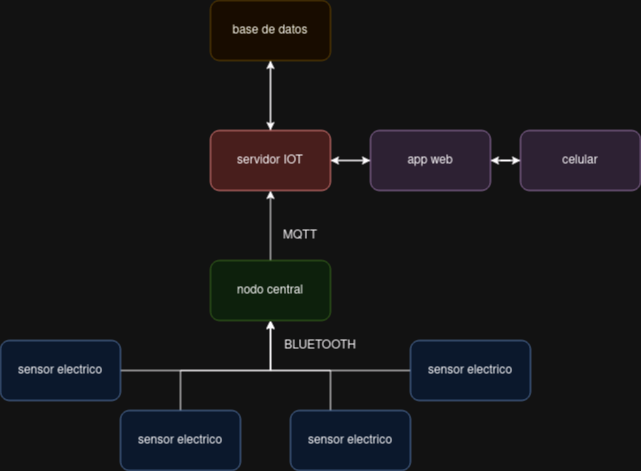
\includegraphics[width=.8\textwidth]{./Figuras/diagBloques.png}
\caption{Diagrama en bloques del sistema.}
\label{fig:diagBloques}
\end{figure}

\vspace{25px}

El usuario final, conectado desde un dispositivo móvil, podrá:

\begin{itemize}
\item{Verificar el consumo eléctrico de la red de dispositivos.
	}
\item{Configurar alarmas de exceso de consumo.
	}
\item{Verificar cortes en el consumo eléctrico.
	}
\item{Calcular el precio diferenciado por fecha y dispositivos.  
	}
\end{itemize}



\newpage

\section{2. Identificación y análisis de los interesados}
\label{sec:interesados}


En el cuadro \ref{tab:interesados} se presentan los interesados en el proyecto. 

\begin{table}[htbp]
\begin{tabularx}{\linewidth}{@{}|l|X|X|l|@{}}
\hline
\rowcolor[HTML]{C0C0C0} 
Rol           & Nombre y Apellido & Organización 	& Puesto 	\\ \hline
%Auspiciante   & Ing. Martin Rodriguez                 &    Soft SA          	&       DBA 	\\ \hline
Cliente       & \clientename      &\empclientename	&       	Director Trabajo final\\ \hline
Responsable   & \authorname       & FIUBA        	& Alumno 	\\ \hline
Colaboradores &   Sr. Gabriel Garcia                &              	&    Desempleado    	\\ \hline
Orientador    & \supname & \pertesupname 	& Director Trabajo final \\ \hline
Equipo        &  Ing. Guillermo Tala          			  &   Soft SA               		      &   Desarrollador  	\\ \hline
Usuario final &  Sra. Ana Alvarez                 &              	&       Jubilada 	\\ \hline
\end{tabularx}
\caption{Identificación de los interesados}
\label{tab:interesados}
\end{table}

\vspace{20px}

Se describen las características de los interesados en el proyecto:

\begin{itemize}
%	\item Auspiciante: esta dispuesto a gastar dinero para el proyecto.
	\item Cliente: tiene experiencia previa en planificación, va a poder ayudar con la definición de los requerimientos y demás detalles. 
	\item Responsable: tiene la responsabilidad y el interes suficiente para terminar el proyecto.
	\item Colaboradores: esta desempleado y tiene el tiempo suficiente para comprar los materiales necesarios, va a poder ayudar mucho en cuestiones de logística.
	\item Orientador: es el especialista en esta tecnología.Se puede tener en cuenta  a la hora de evaluar alternativas.Cumple el rol de auspiciante y cliente ayudando en cuestiones económicas.
	\item Equipo: Es especialista en desarrollo desde hace varios años. Planificar considerando que tiene poco tiempo extra laboral.
	\item Usuario Final: tiene la necesidad de probar el proyecto, por motivos económicos.
\end{itemize}




\section{3. Propósito del proyecto}
\label{sec:proposito}


El propósito de este proyecto es implementar un sistema IoT para monitorear el consumo eléctrico en viviendas y departamentos de un mismo predio.
Se pretende aplicar los conocimientos adquiridos para la gestión del proyecto y el diseño del sistema en todas sus etapas.


\section{4. Alcance del proyecto}
\label{sec:alcance}


El presente proyecto incluye:

\begin{itemize}
\item{Desarrollo de la aplicacion IoT( frontend, backend, base de datos ).}
\item{Desarrollo de firmware para módulos sensor y transmisor }
\item{Desarrollo de un prototipo  para el modulo sensor en protoboard o placa perforada}
\item{Desarrollo de un prototipo para el modulo transmisor ( interface sensores e internet ) en protoboard o placa perforada}
\end{itemize}




El presente proyecto no incluye:

\begin{itemize}
\item{La construcción y/o adaptación del PCB para los módulos sensor y transmisor.}
\item{La construcción y/o adaptación de un gabinete para los módulos sensor y transmisor.}
\item{El desarrollo de una aplicación de celular para sistemas Android o similares}
\end{itemize}




\section{5. Supuestos del proyecto}
\label{sec:supuestos}


Para el desarrollo del presente proyecto se supone que:

\begin{itemize}
\item{El modulo ESP32 tiene suficientes recursos para la implementación de este sistema.}
\item{Se conseguirán los materiales necesarios en el mercado local.}
\item{El diseño y desarrollo de código se realizará en tiempo y forma.}
\item{No se presentarán retrasos debidos a problemas de hardware, por ejemplo, en el diseño e implementación de los módulos sensor y transmisor.}
\item{El país no tendrá una devaluación lo suficientemente grande como para no poder contratar un servicio en la nube para alojar la aplicación.}
\end{itemize}







\section{6. Requerimientos}
\label{sec:requerimientos}

Se detallan los requerimientos necesarios dentro del proyecto:

\begin{enumerate}
	\item Requerimientos funcionales
		\begin{enumerate}
			\item El sistema debe ser capaz de medir el consumo eléctrico por hora, día, semana y mes.
			\item El modulo sensor y el modulo transmisor deben ser alimentados con la tension nominal de 220 Vac o en su defecto por una batería de 12 Vdc.
			\item El sistema debe ser capaz de monitorear el consumo del mismo dispositivo de medición.
			\item El dispositivo funcional debe poder trabajar en un rango de temperatura ambiente de 0°C a 50°C .
			\item El dispositivo funcional debe poder trabajar en un rango de corriente de 0 a 25 A .
			\item El dispositivo funcional debe poder trabajar a una frecuencia de 50 Hz.
			
		\end{enumerate}
		
	\item Requerimientos de documentación
		\begin{enumerate}
			\item La documentación debe contar con un esquemático de circuito eléctrico.
			\item La documentación debe contar con  un diagrama de la aplicación.
			\item La documentación debe contar con un manual de uso.
			\item La documentación debe contar con un manual de instalación.
			\item Informe de avance de proyecto.
			\item Memoria técnica del proyecto.
		\end{enumerate}
		
	\item Requerimiento de testing
		\begin{enumerate}
			\item Se deben realizar pruebas de consumo eléctrico en un domicilio, con al menos dos dispositivos sensores por el período de una semana.
			\item Se deben contrastar las pruebas de consumo eléctrico con el medidor eléctrico del domicilio.
			\item Se debe controlar la correcta activación de las alarmas por exceso de consumo.
			\item Se debe controlar el correcto funcionamiento del dispositivo ante cortes en el suministro eléctrico.
								
		\end{enumerate}
	\item Requerimientos de la interfaz
		\begin{enumerate}
			\item El usuario debe poder configurar y visualizar alarmas por exceso de consumo eléctrico.
			\item El usuario debe poder seleccionar y visualizar el consumo eléctrico general por hora, día, semana y mes.
			\item El usuario debe poder seleccionar y visualizar el consumo eléctrico general promedio.
			\item El usuario debe poder seleccionar y visualizar el consumo eléctrico sensado por cada dispositivo.
			\item El usuario debe poder visualizar los cortes de suministro eléctrico.
			\item El usuario debe poder configurar alarmas por exceso de consumo eléctrico.	
			\item El usuario debe poder controlar el nivel de tension de batería auxiliar del dispositivo y notificar cuando la tension sea baja. 
		\end{enumerate}
	
	\item Requerimientos interoperabilidad
	\begin{enumerate}
		\item Los dispositivos sensores deben poder comunicarse via Bluetooth con el modulo transmisor.
		\item El modulo transmisor debe comunicarse con el servidor web por medio protocolo MQTT.
	\end{enumerate}
	
\end{enumerate}



\section{7. Historias de usuarios (\textit{Product backlog})}
\label{sec:backlog}

Las historias de usuario para el proyecto son las siguientes:

\begin{itemize}

\item{Como administrador  de un departamento necesito saber el consumo eléctrico mensual de cada domicilio para distribuir los gastos equitativamente sobre los inquilinos.}


Dificultad: media (3) → Porque necesita mas dispositivos conectados en un mismo tablero.

Complejidad: baja (1) → Seria la misma implementación que para pocos dispositivos.

Riesgo: medio (3) → No tener el suficiente espacio para conectar todos los dispositivos en un mismo tablero eléctrico.

Story Point: 8 

(3 + 1 + 3 = 7 → 8 es el valor más cercano en Fibonacci)


\item{Como dueño de esta vivienda diariamente necesito saber  si estoy excediendo  el consumo eléctrico de una vivienda tipo, para no incurrir en multas o penalidades.
}

Dificultad: alta (5) → Porque necesita saber los limites de consumo eléctrico de cada empresa para cada mes.

Complejidad: baja (1) → Se podría implementar un alerta automático para el cambio de los limites de consumo por mes. 

Riesgo: medio (3) → No poder actualizar obtener o estimar mensualmente los valores limites de consumo sin penalización. 

Story Point: 13 

(5 + 1 + 3 = 9 → 13 es el valor más cercano en Fibonacci)

\item{Como inquilino me gustaría saber el consumo eléctrico de los electrodomésticos de mi casa para evaluar el remplazo u otra alternativa.
}

Dificultad: media (3) → Porque necesita más dispositivos conectados.

Complejidad: baja (1) → Seria el mismo sistema con mas dispositivos conectados.

Riesgo: alta (5) → El electrodoméstico puede ser que consuma mucha potencia.

Story Point: 13 

(3 + 1 + 5 = 9 → 13 es el valor más cercano en Fibonacci)

\item{Como propietario deseo ver desde el celular los consumos eléctricos para no registrar un control manualmente desde el medidor.}


Dificultad: baja (1) → Porque necesita un solo dispositivo conectado al tablero.

Complejidad: baja (1) → La implementación más sencilla del sistema.

Riesgo: baja (1) → Solo requiere de la implementación de un dispositivo.

Story Point: 3 

(1 + 1 + 1 = 3 → 3 es el valor más cercano en Fibonacci)

\item{Como desarrollador deseo implementar la infraestructura de la aplicación en la nube para hacer mas escalable la aplicación.}


Dificultad: media (3) → Porque se necesitan conocimientos técnicos para la implementación en la nube para no incurrir en gastos innecesarios.

Complejidad: alta (5) → Es un arquitectura relativamente compleja.

Riesgo: medio (3) → No disponer del tiempo y conocimiento suficiente para implementar la aplicación.

Story Point: 13 

(3 + 5 + 3 = 11 → 13 es el valor más cercano en Fibonacci)


\end{itemize}


Para el calculo de los story points se consideraron los siguientes criterios:

\begin{itemize}
\item Se asigno valores de la serie de fibonacci, de acuerdo a la severidad 1 baja, 3 media y 5 alta.
\item Se sumaron los valores de dificultad, complejidad y riesgo para aproximar al numero de la serie de fibonacci mas alto( criterio para no subestimar ) y se asigno ese valor a la story point.
\end{itemize}


\section{8. Entregables principales del proyecto}
\label{sec:entregables}


Los entregables del proyecto son :

\begin{itemize}
	
	\item Esquemáticos del circuito para el modulo sensor y modulo transmisor.
	\item Código fuente del firmware en codigo C, diseñado para la placa ESP32.
	\item Diagrama de la aplicación	IoT.
	\item Código fuente de la aplicación IoT.
	\item Prototipo funcional verificado.	
	\item Manual de instalación.
	\item Manual de uso.
	\item Informe de avance del proyecto.
	\item Memoria técnica del proyecto.
\end{itemize}


\section{9. Desglose del trabajo en tareas}
\label{sec:wbs}

Las tareas a realizar son las siguientes:

\begin{enumerate}
\item Investigación inicial. (40 hs)
	\begin{enumerate}
	\item Investigación sobre proyectos existentes.	(8 hs)
	\item Investigación sobre el modulo sensor con conexión Bluetooth. (8 hs)
	\item Investigación sobre el modulo transmisor con conexión MQTT. (8 hs)
	\item Investigación sobre librerías existentes de la placa ESP32. (8 hs)
	\item Investigación sobre aplicaciones implementadas en la nube. (8 hs)
	\end{enumerate}
\item Materiales necesarios. (44 hs)
	\begin{enumerate}
	\item Identificar los proveedores para los materiales necesarios. (12 hs)
	\item Comprar los materiales.(12 hs)
	\item Identificar los proveedores de servicios en la nube. (12 hs)
	\item Contratar servicios en la nube. (8 hs)
	\end{enumerate}
\item Desarrollo de hardware. (104 hs)
	\begin{enumerate}
	\item Diseño de circuito esquemático en protoboard. (36 hs)
	\item Implementación en protoboard. (24 hs)
	\item Diseño de circuito en placa perforada. (12 hs)
	\item Implementación en placa perforada.(16 hs)
	\item Pruebas individuales del funcionamiento de los módulos. (8 hs)
	\item Pruebas de interconexión entre los módulos. (8 hs)
	\end{enumerate}
\item Desarrollo de firmware. (68 hs)
	\begin{enumerate}
	\item Confección del diagrama de bloques del código. (8 hs)
	\item Desarrollo de código C para la comunicación UART (Bluetooth). (12 hs)
	\item Desarrollo de código C para la comunicación MQTT.	(12 hs)
	\item Desarrollo de código para consumo de batería.	(12 hs)
	\item Pruebas individuales del funcionamiento del firmware de comunicación. (8 hs)
	\item Pruebas de interconexión del firmware. (16 hs)
	\end{enumerate}
\item Desarrollo de aplicación. (124 hs)
	\begin{enumerate}
	\item Confección de un diagrama de la aplicación IoT. (8 hs)
	\item Confección de un diagrama en bloques del código. (8 hs)
	\item Desarrollo del código del frontend. (36 hs)
	\item Desarrollo del código del backend. (36 hs)
	\item Integración de la aplicación en la nube. (12 hs)
	\item Pruebas individuales del funcionamiento del backend y frontend. (8 hs)
	\item Pruebas de interconexión del backend y frontend. (16 hs)
	\end{enumerate}

\item Etapa de integración. (48 hs)
	\begin{enumerate}
	\item Integración de software y  hardware. (24 hs)
	\item Pruebas generales de software y  hardware. (24 hs)
	\end{enumerate}
	
\item Testing del proyecto. (36 hs)
	\begin{enumerate}
	\item Instalación del sistema en un domicilio. (8 hs)
	\item Pruebas de consumo eléctrico en un domicilio.	(4 hs)
	\item Pruebas del dispositivo ante cortes de suministro eléctrico.	(4 hs)
	\item Pruebas del sistema de alarmas del dispositivo. (4 hs)
	\item Pruebas de duración de la batería. (16 hs)
	\end{enumerate}
	
\item Verificación del prototipo. (8 hs)
	\begin{enumerate}
	\item Verificación de la interfaz de usuario. (8 hs)
	\end{enumerate}	
	
\item Documentación. (153 hs)
	\begin{enumerate}
	\item Documentación de esquemáticos. (4 hs)
	\item Documentación del código C. (8 hs)
	\item Documentación de la aplicación IoT. (8 hs)
	\item Documentación del manual de instalación. (8 hs)
	\item Documentación del manual de uso. (8 hs)
	\item Informe de avance del proyecto. (20 hs)
	\item Memoria técnica del proyecto. (97 hs)

	\end{enumerate}


\end{enumerate}

Cantidad total de horas: (625 hs)

\newpage

\section{10. Diagrama de Activity On Node}
\label{sec:AoN}


Se puede ver el AON en la figura \ref{fig:AoN}, el mismo se confecciono teniendo en cuenta que las tareas :

\begin{figure}[htpb]
\centering 
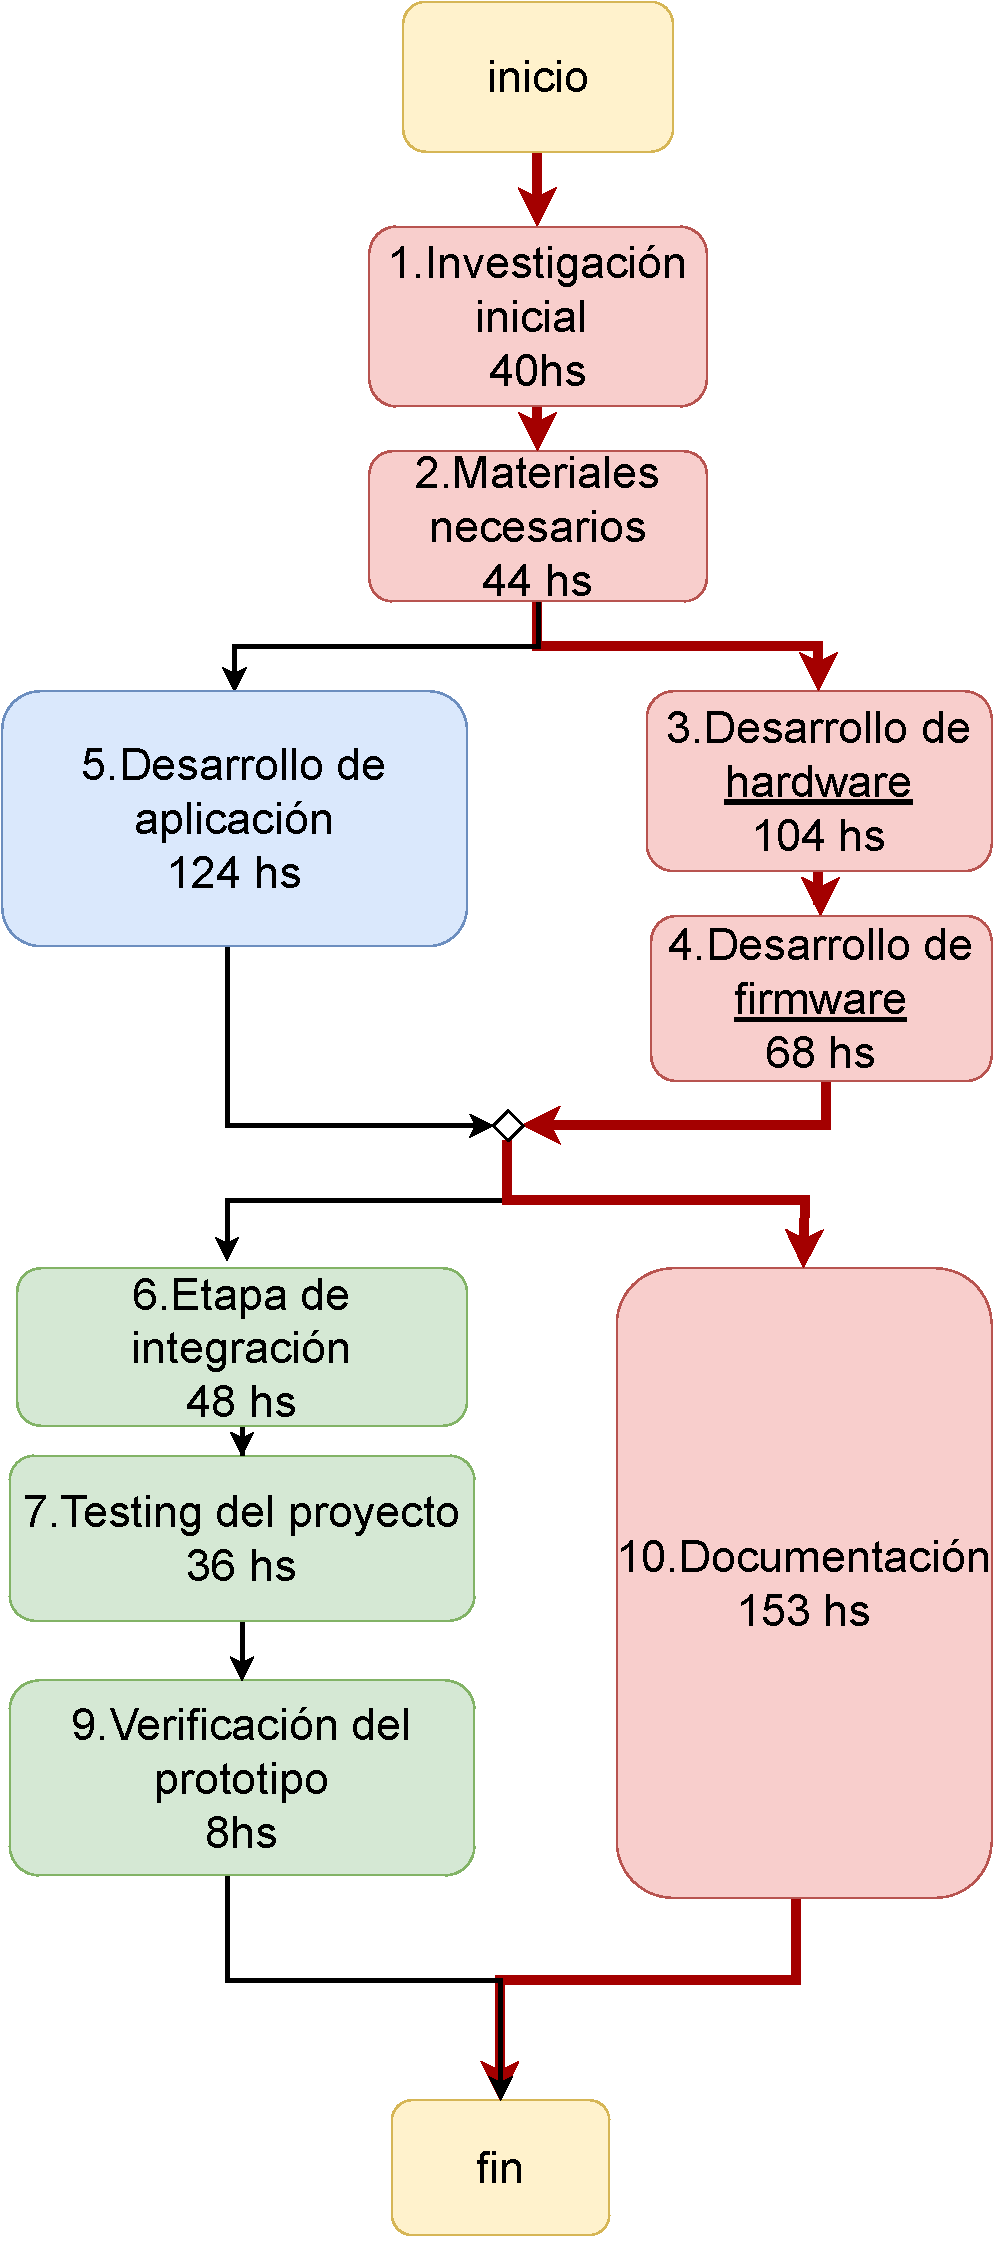
\includegraphics[width=0.5 \textwidth, height=1.1 \textwidth]{./Figuras/AON.pdf}
\caption{Diagrama de \textit{Activity on Node}.}
\label{fig:AoN}
\end{figure}


Observando  la figura  \ref{fig:AoN} se determinan las siguientes cuestiones:

\begin{itemize}
	\item Las subtareas son todas secuenciales  de acuerdo al orden establecido en la seccion \ref{sec:wbs}.
	\item El camino critico se indica con las tareas de color rojo,  flechas de color rojo y trazo grueso. La cantidad de horas para finalizar el proyecto por el camino critico es de 348 hs.
	\item El desarrollo de la aplicación marcado en azul puede demorarse hasta 48 hs respecto del camino critico.
	\item El desarrollo de las tareas de integración, testing del proyecto y verificación del proyecto marcado en verde puede demorarse hasta 61 hs respecto del camino critico.
	

\end{itemize}
	


\section{11. Diagrama de Gantt}
\label{sec:gantt}

En la figura \ref{fig:gantt}, se muestra el diagrama de Gantt del proyecto construido en gantter:


\begin{figure}[htpb]
\centering 
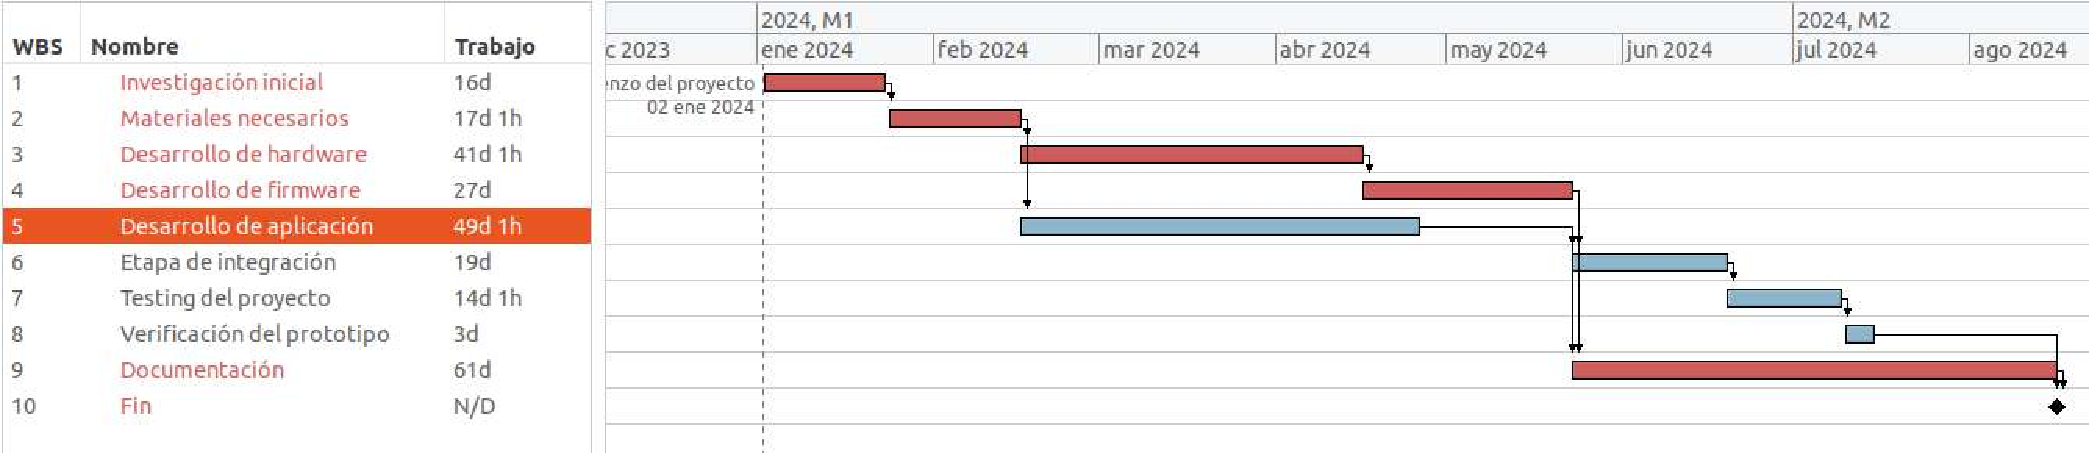
\includegraphics[width=1.0\textwidth, height=.43 \textwidth]{./Figuras/ganttProyecto.pdf}
\caption{Diagrama de Gantt del proyecto.}
\label{fig:gantt}
\end{figure}

Para construir el diagrama de gantt del proyecto se realizaron las siguientes consideraciones:

\begin{itemize}
\item Se establecen  2.5 h de trabajo diario por tarea.
\item Se establecen  los días laborables de lunes a viernes.
\item Se establecen  los días no laborables los sábados y domingos.
\item El camino critico es el establecido en color rojo.
\item El proyecto empieza el día 02/01/2024 y finaliza el 13/08/2024.
\item Se tomaron los grupos de tareas generales para confeccionar el diagrama de Gantt de la figura \ref{fig:gantt}, dado que las tareas internas son secuenciales como se puede ver en los diagramas de gantt ampliado de las figuras \ref{fig:gantt1}, \ref{fig:gantt2} y \ref{fig:gantt3}.
\end{itemize}



\begin{figure}[htpb]
\centering 
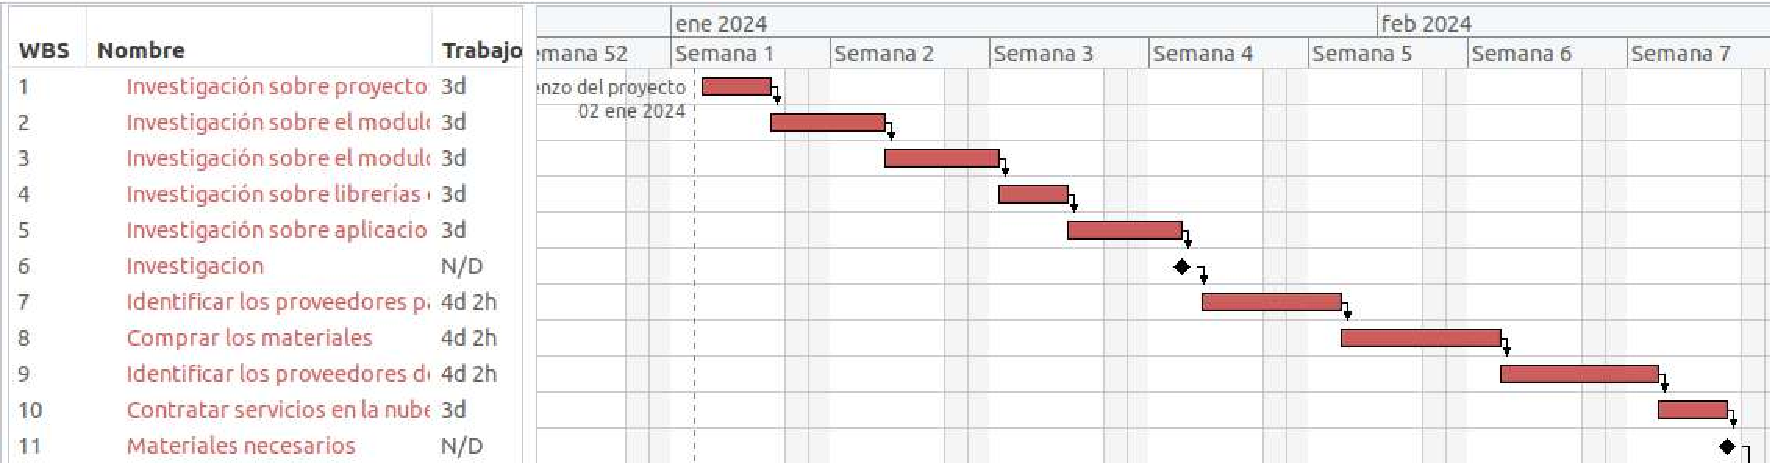
\includegraphics[width=1.0\textwidth, height=.43 \textwidth]{./Figuras/ganttProyecto1.pdf}
\caption{Diagrama de Gantt de la etapa de Investigación y Materiales necesarios.}
\label{fig:gantt1}
\end{figure}


\begin{figure}[htpb]
\centering 
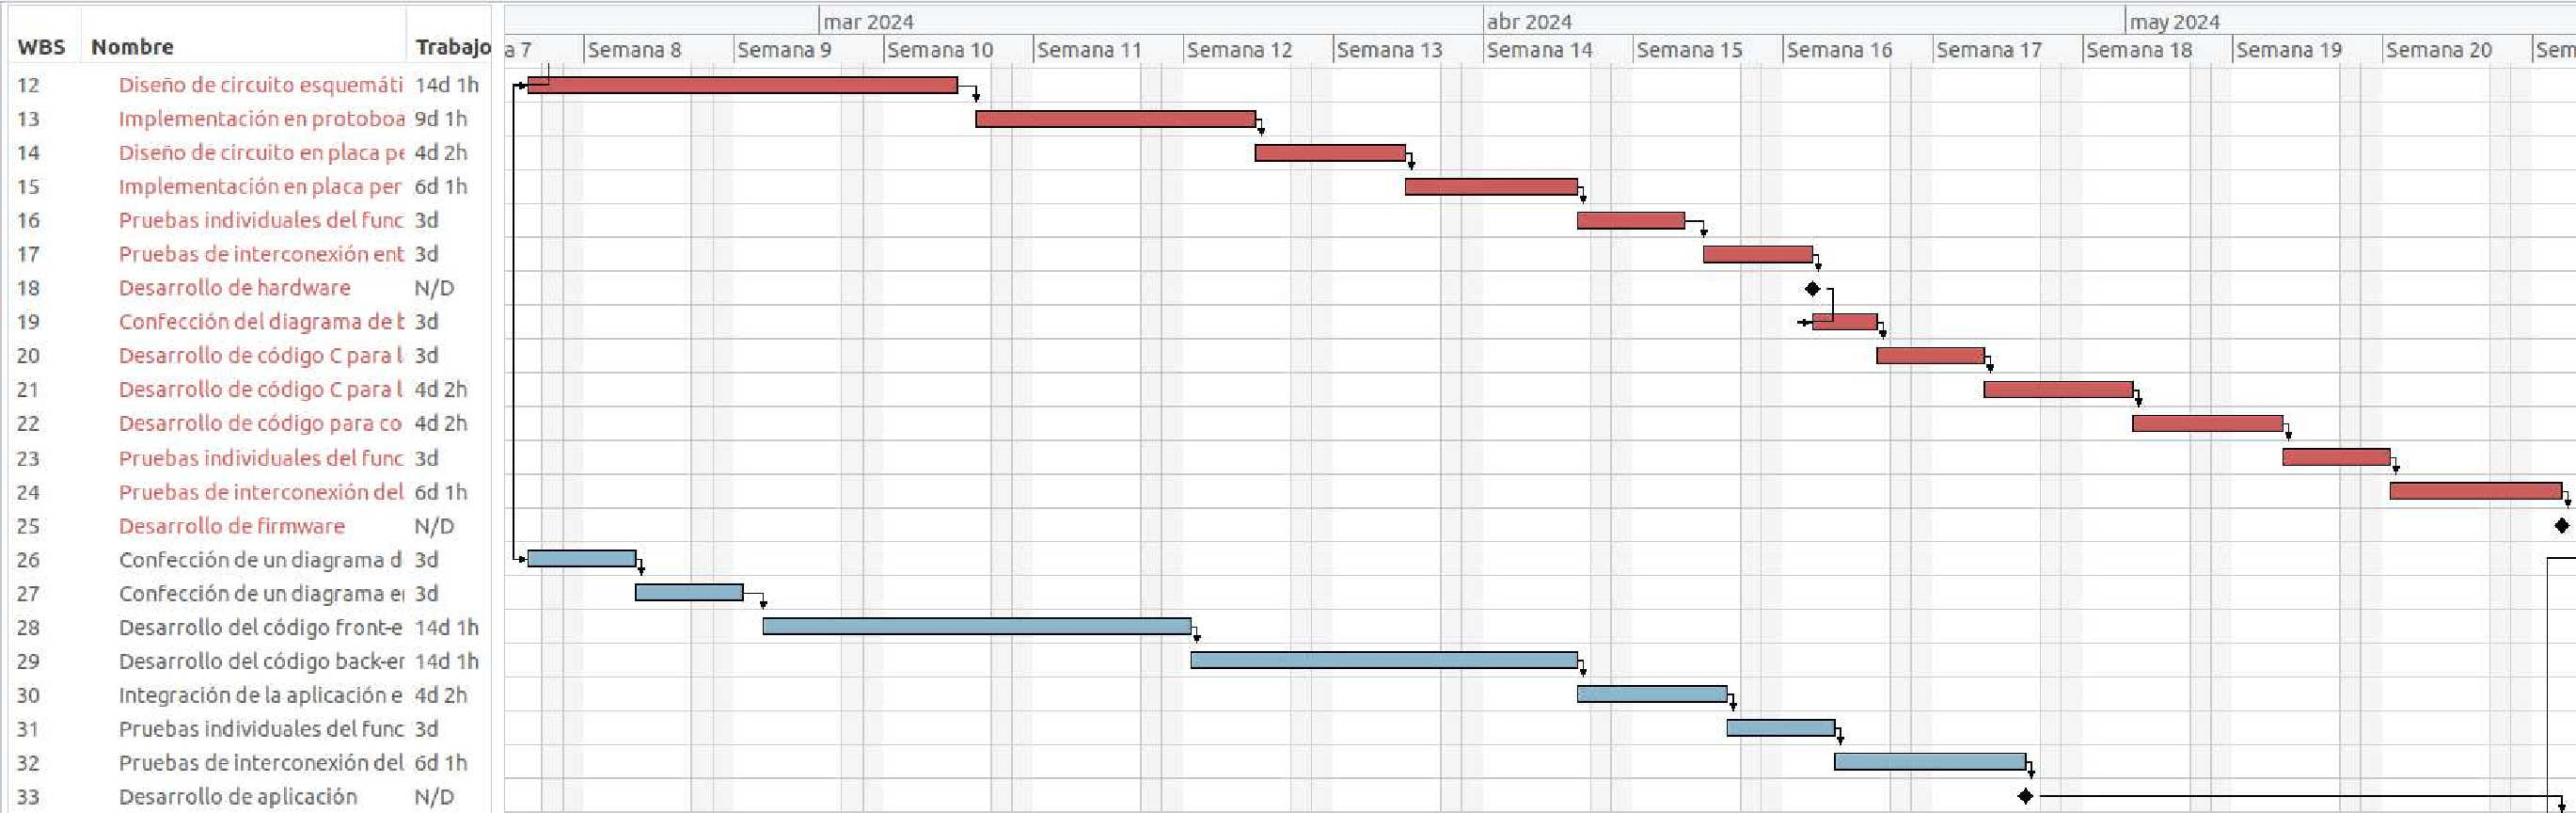
\includegraphics[width=1.0\textwidth, height=.43 \textwidth]{./Figuras/ganttProyecto2.pdf}
\caption{Diagrama de Gantt de la etapa de Desarrollo de hardware, Desarrollo de firmware y Desarrollo de aplicación.}
\label{fig:gantt2}
\end{figure}


\begin{figure}[htpb]
\centering 
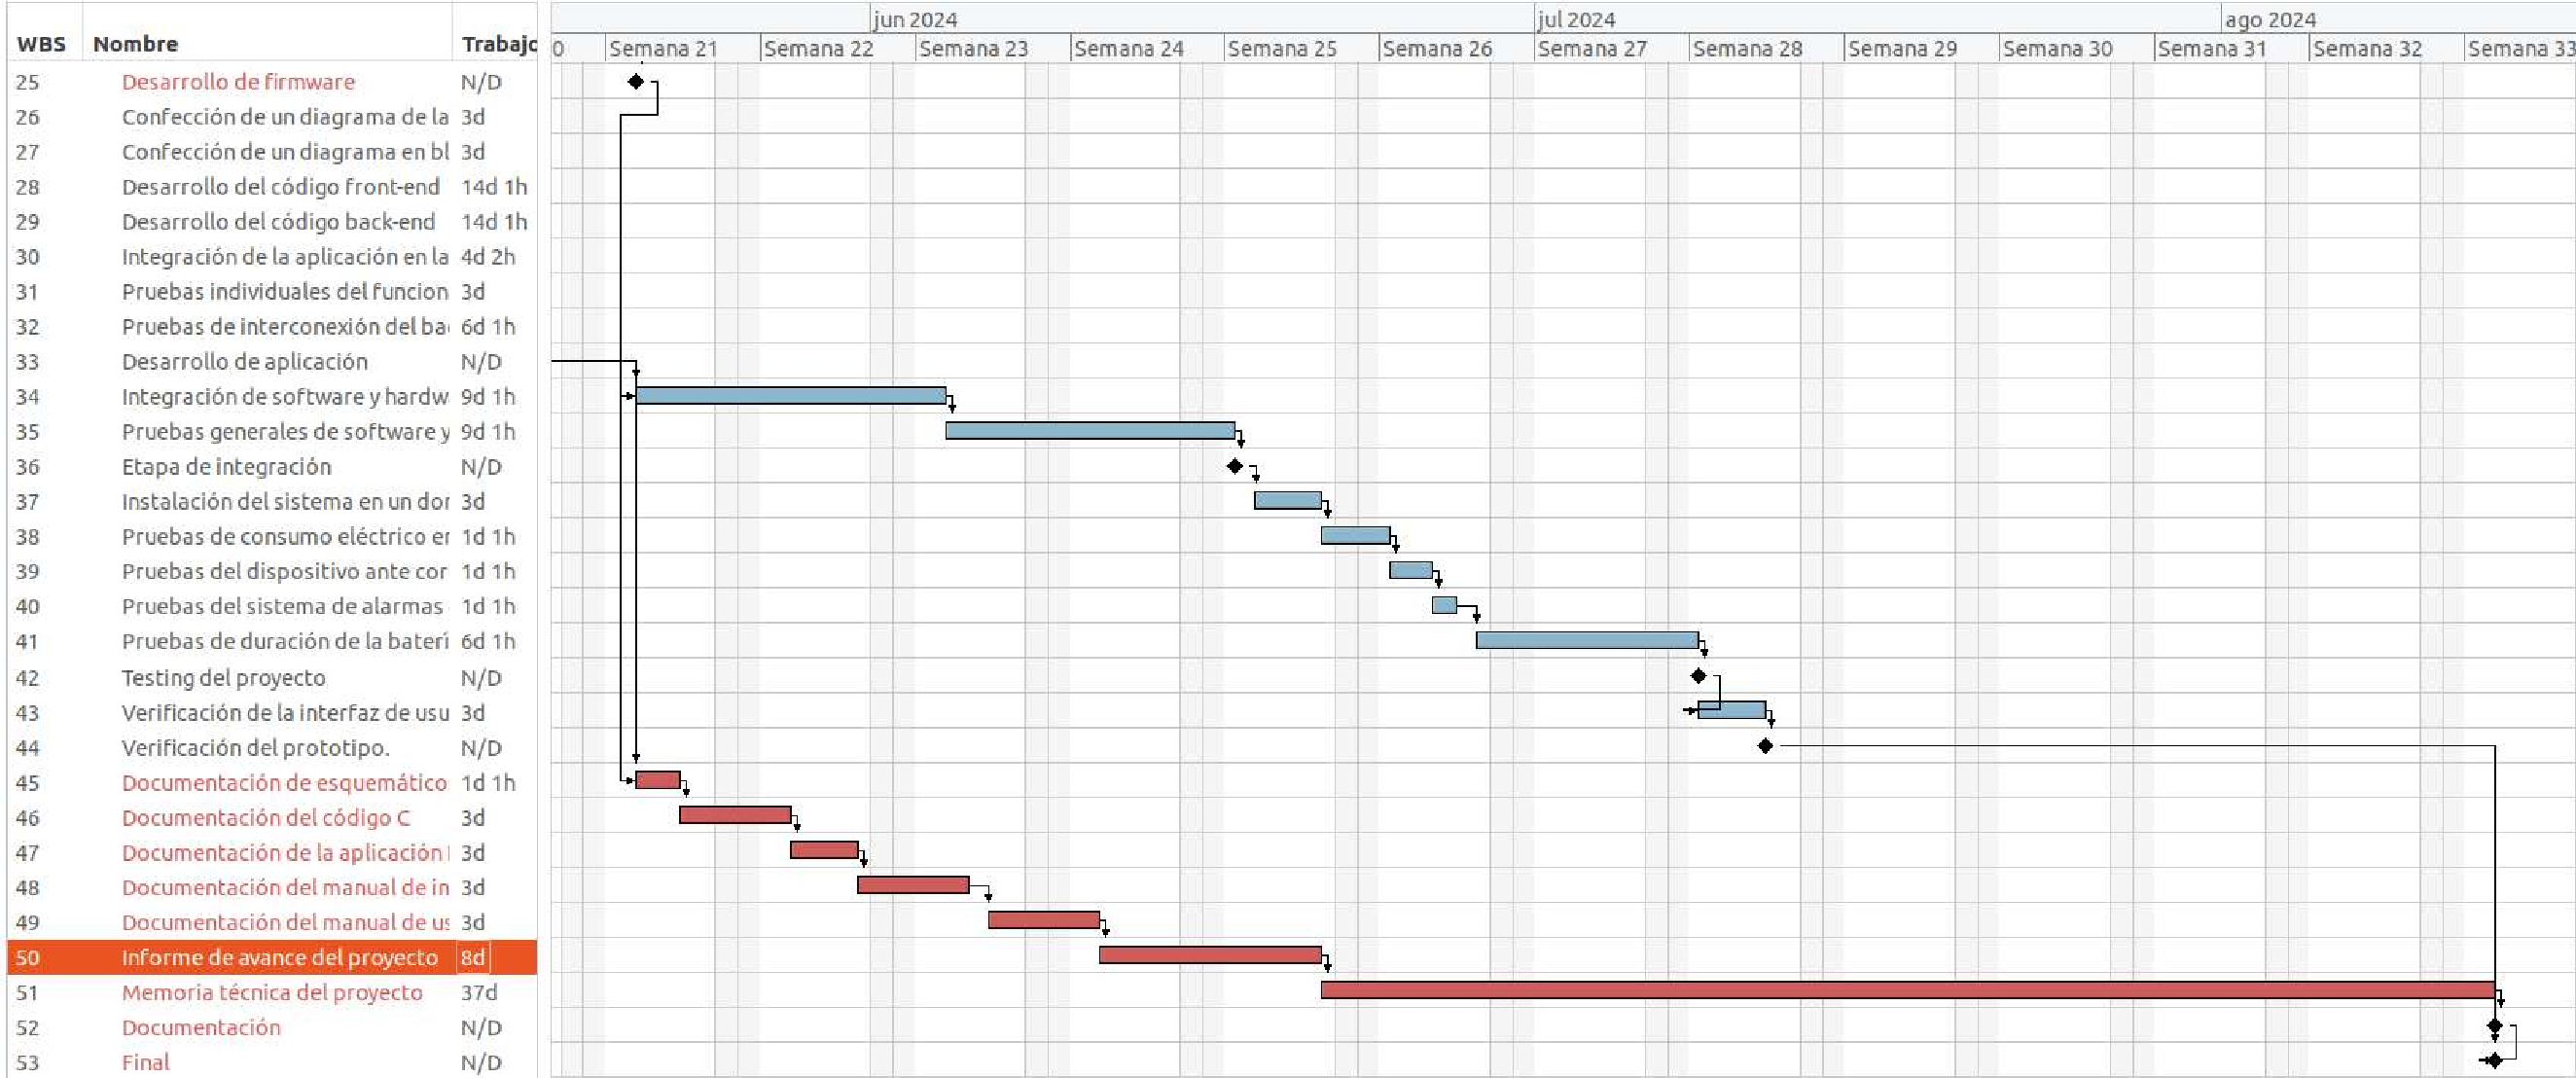
\includegraphics[width=0.98\textwidth, height=.43 \textwidth]{./Figuras/ganttProyecto3.pdf}
\caption{Diagrama de Gantt de la Etapa de integración, Testing del proyecto, Verificación del prototipo y Documentación.}
\label{fig:gantt3}
\end{figure}



\section{12. Presupuesto detallado del proyecto}
\label{sec:presupuesto}



En el cuadro \ref{tab:costos} se presentan los costos del proyecto. 



\begin{table}[htpb]
\centering
\begin{tabularx}{\linewidth}{@{}|X|c|r|r|@{}}
\hline
\rowcolor[HTML]{C0C0C0} 
\multicolumn{4}{|c|}{\cellcolor[HTML]{C0C0C0}COSTOS DIRECTOS} \\ \hline
\rowcolor[HTML]{C0C0C0} 
Descripción &
  \multicolumn{1}{c|}{\cellcolor[HTML]{C0C0C0}Cantidad} &
  \multicolumn{1}{c|}{\cellcolor[HTML]{C0C0C0}Valor unitario} &
  \multicolumn{1}{c|}{\cellcolor[HTML]{C0C0C0}Valor total} \\ \hline
  
  \multicolumn{1}{|l|}{Horas de ingeniería}  &
  \multicolumn{1}{c|}{625 h} &
  \multicolumn{1}{c|}{3000 \$} &
  \multicolumn{1}{c|}{1875000 \$} \\ \hline
 
 \multicolumn{1}{|l|}{Materiales}  &
  \multicolumn{1}{c|}{2 prototipos} &
  \multicolumn{1}{c|}{100000 \$} &
  \multicolumn{1}{c|}{200000 \$} \\ \hline
  
  \multicolumn{1}{|l|}{Servicios en la Nube}  &
  \multicolumn{1}{c|}{6 meses} &
  \multicolumn{1}{c|}{17000 \$} &
  \multicolumn{1}{c|}{102000 \$} \\ \hline

  
\multicolumn{3}{|c|}{SUBTOTAL} &
  \multicolumn{1}{c|}{2177000 \$} \\ \hline
\rowcolor[HTML]{C0C0C0} 
\multicolumn{4}{|c|}{\cellcolor[HTML]{C0C0C0}COSTOS INDIRECTOS} \\ \hline
\rowcolor[HTML]{C0C0C0} 
Descripción &
  \multicolumn{1}{c|}{\cellcolor[HTML]{C0C0C0}Cantidad} &
  \multicolumn{1}{c|}{\cellcolor[HTML]{C0C0C0}Valor unitario} &
  \multicolumn{1}{c|}{\cellcolor[HTML]{C0C0C0}Valor total} \\ \hline


\multicolumn{1}{|l|}{Viáticos}  &
  \multicolumn{1}{c|}{154 días} &
  \multicolumn{1}{c|}{3000 \$} &
  \multicolumn{1}{c|}{462000 \$} \\ \hline
  
\multicolumn{1}{|l|}{Alquiler de taller}  &
 \multicolumn{1}{c|}{8 meses} &
  \multicolumn{1}{c|}{60000 \$} &
  \multicolumn{1}{c|}{480000 \$} \\ \hline
  
\multicolumn{3}{|c|}{SUBTOTAL} &
  \multicolumn{1}{c|}{942000 \$} \\ \hline
\rowcolor[HTML]{C0C0C0}
\multicolumn{3}{|c|}{TOTAL} &
\multicolumn{1}{c|}{3119000 \$} 
   \\ \hline
\end{tabularx}%
\caption{Cuadro de costos.}
\label{tab:costos}
\end{table}


Para construir el cuadro \ref{tab:costos} del proyecto se realizaron las siguientes consideraciones:

\begin{itemize}
\item Horas de ingeniería: se calculo respecto del sueldo  mensual  $\frac{720000}{30\  dias\ \* 8\ h } \approx 3000\$ $
\item Materiales: se calculo el valor correspondiente para la placa perforada, protoboard, cables , microcontroladores y un 20 \% mas de estimación.
\item Servicio en la nube: se tomo el valor mensual en el servicio de la pagina hostinger. Se tiene en cuenta que solo 6 meses, dado que los primeros dos meses no se realizan pruebas en la nube.
\item Viáticos: se considera el consumo de alimentos promedio en un día.
\item Alquiler de taller: comprenden los costos de alquiler y de consumo eléctrico por mes.
\end{itemize}


\section{13. Gestión de riesgos}
\label{sec:riesgos}

Los riesgos identificados en el proyecto son los siguientes:


Riesgo 1: no conseguir los componentes de hardware necesarios  para el proyecto.
\begin{itemize}
	\item Severidad (S): 8, debido a que los componentes de hardware son necesarios para la implementación del proyecto en los plazos de tiempo estipulados. 
	\item Ocurrencia (O):3, debido a que los componentes son productos de alta demanda en el mercado local.
\end{itemize}

Riesgo 2: comprar un componente defectuoso o roto.
\begin{itemize}
	\item Severidad (S): 5, porque es necesario el correcto funcionamiento de los componentes  para la integración de los mismos al proyecto.
	\item Ocurrencia (O): 1,porque los componentes utilizados tiene un control de calidad muy alto.
\end{itemize}

Riesgo 3: exceso en los tiempos de trabajo.
\begin{itemize}
	\item Severidad (S): 10, de no cumplirse con los tiempos se pondría en riesgo la finalización del proyecto en el tiempo planificado. 
	\item Ocurrencia (O): 4, porque hay desarrollos sobre los que no se tienen conocimientos, o el conocimiento es bajo.
\end{itemize}


Tabla de gestión de riesgos:      (El RPN se calcula como RPN=SxO)

\begin{table}[htpb]
\centering
\begin{tabularx}{\linewidth}{@{}|X|c|c|c|c|c|c|@{}}
\hline
\rowcolor[HTML]{C0C0C0} 
Riesgo & S & O & RPN & S* & O* & RPN* \\ \hline
No conseguir los componentes de hardware necesarios  para el proyecto       & 8  & 3  &  24   & 8  &  1  &  8      \\ \hline
Comprar un componente defectuoso o roto       & 5  & 1  &  5   &  5  & 1  &  5    \\ \hline
Exceso en los tiempos de trabajo       & 10  & 4  &  40   &   10 &  1 & 10     \\ \hline
\end{tabularx}%
\end{table}

Criterio adoptado: 
se tomarán medidas de mitigación en los riesgos cuyos números de RPN sean mayores a 20.

Nota: los valores marcados con (*) en la tabla corresponden luego de haber aplicado la mitigación.


Plan de mitigación de los riesgos que originalmente excedían el PRN máximo establecido:
 
Riesgo 1: no conseguir los componentes de hardware necesarios  para el proyecto en los locales de venta. Para mitigar este riesgo se realizará el correspondiente encargo de los componentes necesarios con suficiente antelación 


Severidad (S): 8, debido a que los componentes de hardware son necesarios para la implementación del proyecto en los plazos establecidos.  

Probabilidad de Ocurrencia (O):  1, debido a que los componentes son productos de alta demanda en el mercado local.
 
Riesgo 3: exceso en los tiempos de trabajo. Para mitigar este riesgo se planificará de manera apropiada la estipulación de tiempos para cada tarea del proyecto

Severidad (S): 10, de no cumplirse con los tiempos se pondría en riesgo la finalización del proyecto en el tiempo planificado. 

Probabilidad de Ocurrencia (O): 1, porque hay desarrollos sobre los que no se tienen conocimientos, o el conocimiento es bajo.



\section{14. Gestión de la calidad}
\label{sec:calidad}


\begin{enumerate}
	\item Requerimientos funcionales
		\begin{itemize}

			\item El sistema debe ser capaz de medir el consumo eléctrico por hora, día, semana y mes.

			\begin{itemize}
			\item Verificación: se medirá el consumo eléctrico y se contrastará con las mediciones de un multímetro eléctrico y una pinza amperímetrica.
			\item Validación: el cliente verificará el consumo eléctrico y contratará el valor con el medidor eléctrico de su domicilio.
			\end{itemize}

	\item El modulo sensor y el modulo transmisor deben ser alimentados con la tension nominal de 220 Vac o en su defecto por una batería de 12 Vdc.
			
			\begin{itemize}
		\item Verificación: se verificará el correcto funcionamiento del sistema con los módulos alimentados a 220Vac y con una batería de 12 Vdc.
			\item Validación: El cliente probará el dispositivo instalado en su domicilio.
			\end{itemize}
			
		\end{itemize}
		
	\item Requerimientos de documentación
		\begin{itemize}

		\item La documentación debe contar con un manual de instalación.
			
		\begin{itemize}
		\item Verificación: se verificarán los pasos de instalación siguiendo el manual, en caso de  corresponder se rectificara el mismo. 
		\item Validación: se instalara un prototipo, siguiendo los pasos detallados en el manual y se corroborara el correcto funcionamiento del sistema.
		\end{itemize}
			
		\item La documentación debe contar con un manual de uso.
		
		\begin{itemize}
		\item Verificación: se verificarán los casos de uso típicos del manual con el sistema en funcionamiento.
		\item Validación: se pedirá a los usuarios utilizar el sistema consultando el manual de uso.
		\end{itemize}
		
		\end{itemize}
		
		
		
	
			
	\item Requerimiento de testing
		\begin{itemize}
		\item Se deben realizar pruebas de consumo eléctrico en un domicilio, con al menos dos dispositivos sensores por el período de una semana.
			\begin{itemize}
			\item Verificación: se verificará la correcta comunicacion de los modulos por Bluetooth, como asi tambien el correcto funcionamiento del protocolo MQTT.
			\item Validación: se pedirá al usuario utilizar el sistema.
			\end{itemize}
			
		\item Se deben contrastar las pruebas de consumo eléctrico con el medidor eléctrico del domicilio.
			\begin{itemize}
			\item Verificación: se verificará el consumo eléctrico de cada modulo, midiendo la potencia desde los dispositivos y se contrastara con el consumo del medidor eléctrico.
			\item Validación: se pedirá al usuario que corrobore que la medición de consumo eléctrico sea la misma que se visualiza en el medidor eléctrico.
			\end{itemize}
		\item Se debe controlar la correcta activación de las alarmas por exceso de consumo.
		\begin{itemize}
			\item Verificación: se configuraran alarmas por exceso de consumo eléctrico. Luego se verificará la correcta activación de las mismas comparando el consumo del medidor eléctrico.
			\item Validación: se pedirá al usuario la configuración de una alarma de exceso de consumo y se verificará la activación desde el sistema. 
			\end{itemize}				
		\end{itemize}
	\item Requerimientos de la interfaz
		\begin{itemize}
			\item El usuario debe poder seleccionar y visualizar el consumo eléctrico general por hora, día, semana y mes.
				\begin{itemize}
			\item Verificación: desde la aplicación se verificará el consumo eléctrico por cada periodo temporal y se contrastara con el consumo visualizado desde el medidor.
			\item Validación: desde la aplicación se pedirá al usuario la selección y visualización del consumo eléctrico para cada periodo temporal.
			\end{itemize}
			
			\item El usuario debe poder configurar alarmas por exceso de consumo eléctrico.	
			\begin{itemize}
			\item Verificación: se configuraran alarmas por exceso de consumo desde la aplicación y se corroborara su correcto funcionamiento por simulación de valores.
			\item Validación: instalado el sistema se pedirá al usuario la configuración de alarmas de alarmas.
			\end{itemize}
		 
		\end{itemize}
	
	\item Requerimientos interoperabilidad
	\begin{itemize}
		\item Los dispositivos sensores deben poder comunicarse via Bluetooth con el módulo transmisor.
		
	\end{itemize}
		\begin{itemize}
			\item Verificación: se verificará la comunicación de los módulos, conectando los mismos y simulando el envió de mensajes por Bluetooth.
			\item Validación: se instalara el sistema y se pedirá al usuario que visualice el consumo eléctrico desde el sistema.
			\end{itemize}
	
\end{enumerate}



\section{15. Procesos de cierre}    
\label{sec:cierre}



Luego de finalizar el proyecto se realizará una reunión final de evaluación , que contemplara las siguientes actividades:

\begin{itemize}
	\item El {\authorname}  estará a cargo de verificar y registrar en un archivo de texto si se respetaron los tiempos establecidos para las tareas del proyecto, si fueron necesarias las pruebas realizadas para satisfacer las expectativas del cliente y las posibles mejoras para una posterior actualización del proyecto.
	\item Se verificará si fue apropiado utilizar los protocolos de comunicación Bluetooth y MQTT frente a otros protocolos de comunicación( ventajas y desventajas), la implementación de la aplicación en la nube frente a la arquitectura on premise y la implementación de sensores y demás componentes físicos del prototipo frente a otras alternativas mas económicas en el mercado.
	Las tareas antes mencionadas estarán a cargo de {\authorname} y supervisadas por \supname. Las mismas deben registrarse en un archivo de texto para futuras mejoras o actualizaciones del proyecto.
	\item El acto de agradecimiento estará organizado y financiado por el  {\authorname}. El acto tendrá por fin agradecer al Director del Trabajo final  {\supname} por el apoyo económico y de desarrollo, al Sr. Gabriel Garcia por el apoyo logístico brindado, al 
Ing. Guillermo Tala  por ser el apoyo fundamental en la etapa de software y a la  Sra. Ana Álvarez  por brindar el lugar para realizar las pruebas del proyecto.
\end{itemize}	  
	  

\end{document}
